\documentclass[a4paper,12pt]{ctexart} %A4纸,小四号字体
\usepackage{ctex}

\usepackage{geometry} 
\geometry{left=2.50cm,right=2.50cm,top=2.50cm,bottom=2.50cm} %上下左右空白距离
\pagestyle{plain}
\usepackage{titlesec} %标题
\usepackage{setspace}
\usepackage{parskip} % Package to tweak paragraph skipping 
\usepackage{tikz} % Package for drawing 
\usepackage{amssymb}%数学字体与符号 
\usepackage{amsmath}%数学公式
 
\usepackage{colortbl} %给表格着色
\usepackage{arydshln} 
\usepackage{multirow} 
\usepackage{multicol}


\usepackage[colorlinks,
            linkcolor=black,
            anchorcolor=black,
            citecolor=black
            ]{hyperref}%超链接与其他 PDF 专有功能(如表单制做)常用 
\usepackage{booktabs}%使用三线表booktabs 
\usepackage{longtable}%长表格自动分页 
\usepackage{graphicx}%插入图片 
\usepackage{float}%将图片插入指定位置[H] 
\usepackage{subcaption} %多张图片组合命名
\usepackage{indentfirst}%首行缩进
\setlength{\parindent}{2em} %段首缩进
\setlength{\parskip}{0em} %段落间距
\usepackage{times} %使得英文默认字体都是Times New Roman
\usepackage{verbatim}
\usepackage{gensymb}
\linespread{1.2} %全文行间距
\usepackage{listings} %matlab宏包
\usepackage{textcomp} %matlab宏包
\usepackage[framed,numbered,autolinebreaks,useliterate]{mcode} %matlab宏包
\usepackage{pythonhighlight} %python宏包
\usepackage{mdframed} %使用引理盒子
\mdfdefinestyle{figstyle}{
  linecolor=black!10,
  backgroundcolor=black!15,
  innertopmargin=10pt,
  innerleftmargin=15pt,
  innerrightmargin=15pt,
  innerbottommargin=10pt
}
\usepackage{enumitem}%有序表无序表间距
\setenumerate[1]{itemsep=0pt,partopsep=0pt,parsep=\parskip,topsep=5pt,leftmargin=19pt}
\setitemize[1]{itemsep=0pt,partopsep=0pt,parsep=\parskip,topsep=5pt,leftmargin=19pt}
\setdescription{itemsep=0pt,partopsep=0pt,parsep=\parskip,topsep=5pt,leftmargin=19pt}


\newcommand{\song}{\CJKfamily{song}}

\titlespacing*{\section} {0pt}{3pt}{6pt} %一级标题间距
\titlespacing*{\subsection} {0pt}{0pt}{0pt} %二级标题间距
\titlespacing*{\subsubsection} {0pt}{0pt}{0pt} %三级标题间距
%\titleformat{\section}[block]{\centering\large\bfseries}{\arabic{section}}{1em}{}
%\titleformat{\subsection}[block]{\normalsize\bfseries}{\arabic{section}.\arabic{subsection}}{0.5em}{}
%章节序号与标题的字号及间距修改
%\titleformat{\subsubsection}[block]{\small\bfseries}{\arabic{section}.\arabic{subsection}.\arabic{subsubsection}}{0.5em}{}

\titleformat{\section}[block]{\centering\Large\heiti\bfseries}{\arabic{section}}{1em}{}
\titleformat{\subsection}[block]{\large\heiti}{\arabic{section}.\arabic{subsection}}{0.5em}{}
%章节序号与标题的字号及间距修改
\titleformat{\subsubsection}[block]{\normalsize\heiti}{\arabic{section}.\arabic{subsection}.\arabic{subsubsection}}{0.5em}{}



\bibliographystyle{plain}

% \setCJKmainfont{SimSun}[AutoFakeBold,ItalicFont=KaiTi]  %伪粗体

\let\heiti\relax
\newCJKfontfamily\heiti{SimHei}[AutoFakeBold]
\setCJKsansfont{SimHei}[AutoFakeBold]

\let\songti\relax
\newCJKfontfamily\songti{SimSun}[AutoFakeBold]
\setCJKmainfont{SimSun}[AutoFakeBold]  %伪粗体


\begin{document}
    \begin{center}
        {\heiti \Large  我的第一份建模终于可以引用了!!附录也写好了!!\\[10pt]} 

        {\heiti \large  摘要\\[10pt]}
    \end{center}
    \setlength\parindent{2em} %%首行缩进2字符
    
     %%从这里写摘要
    本次建模的主要目的有某某某,\textbf{为了测试这次模板的效果,我专门打了好几行字,所以看起来有点啰嗦。}

    这是摘要的第二段,我想看看第二段的效果,所以我又打了一遍,额呵呵呵不过确实没啥好说的,虽然不是词穷。
    

    \setlength\parindent{0em} %%首行缩进0字符

    {\heiti \normalsize 关键词:}{{\small 关键词1\quad  关键词2\quad   关键词3}}

    \newpage

    \section{问题重述}

    \setlength\parindent{2em}
    %%从这里写
    
    请看下面的图\ref{fig:sample-figure-a}、\ref{fig:sample-figure-b}、\ref{fig:sample-figure-c}。

    \begin{figure}[H]
        \centering
        \begin{minipage}[c]{0.3\textwidth}
            \centering
            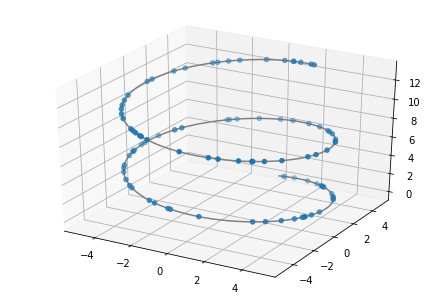
\includegraphics[width=1.05\textwidth]{figtwo.png}
            \subcaption{三维图1}
            \label{fig:sample-figure-a}
        \end{minipage}
        \begin{minipage}[c]{0.3\textwidth}
            \centering
            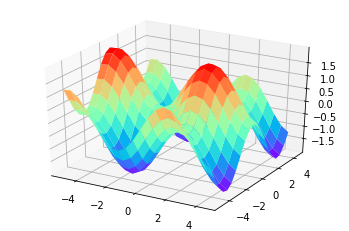
\includegraphics[width=1.05\textwidth]{figthree.png}
            \subcaption{三维图2}
            \label{fig:sample-figure-b}
        \end{minipage}
        \begin{minipage}[c]{0.3\textwidth}
            \centering
            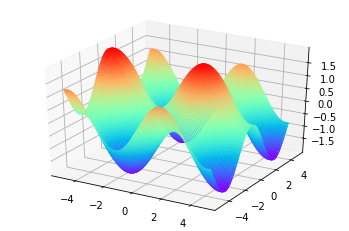
\includegraphics[width=1.05\textwidth]{figfour.png}
            \subcaption{三维图3}
            \label{fig:sample-figure-c}
        \end{minipage}
        \caption{三图并排示例}
        \label{fig:sample-figure}
    \end{figure}
    
    

    请看上面的图\ref{fig:sample-figure}。
    

    \section{问题分析}
    
    \subsection{问题一}
    \subsubsection{问题一的详解}
    \setlength\parindent{2em} %%首行缩进2字符
    
    
    问题一我们的想法是某某某,为了测试这次模板的效果,我专门打了好几行字,所以看起来有点啰嗦。

    这是问题一的第二段,我想看看第二段的效果,所以我又打了一遍,额呵呵呵不过确实没啥好说的,虽然不是词穷。

    \begin{figure}[!h]
        \centering
        
\includegraphics[width=0.90\textwidth]{figone.png}
        \caption{这是一张图}
        \label{fig:thisisafig}
    \end{figure}
    所述信息如图\ref{fig:thisisafig}所示。


    为了测试下面这个有序表的缩进效果,我决定输入两段文字从而实现我需要的文字效果但显然现在还不够长,哦这样就好了。


    \begin{itemize}
	   \label{wuxubiao:001}
        \item 第一项假设,为了查看这条假设的换行效果,根据大学物理学的知识引入质能方程$E=MC^2$来测试这个环境。
        \item 第二项假设
        \item 第三项假设
	   \item ...
    \end{itemize}
    
    
    这是一个无序表\ref{wuxubiao:001}。\cite{bib:one}

    \begin{enumerate}
        \item 第一项假设,为了查看这条假设的换行效果,根据大学物理学的知识引入质能方程$E=mc^2$来测试这个环境。
        \item 第二项假设
        \item 第三项假设
	   \item ...
    \end{enumerate}
    
    这是一个有序表。

    
    接下来将会引入一个引理\ref{box:001}。\\


    \begin{mdframed}[style=figstyle] %一条一条的引理盒子(这个叫提示框。。
        \begin{enumerate}
	   \label{box:001}
            \item \small Initialization: Set $y_v = 0$ for all $v\in N$. Set $T$ to have only $s$.
            \item While $T$ is not a spanning tree...
            \item  \qquad Pick $uv\in \delta(N(T))$ such that $\overline{w_{uv}} = \min \{ \overline{w_e} : e\in \delta(N(T)) \}$.
            \item \qquad $y_w := y_w + \overline{w_{uv}}$ for all $w\in N\setminus N(T)$.
            \item \qquad Add $uv$ and $v$ to $T$.
        \end{enumerate}
    \end{mdframed}

    \begin{equation}
        [x_{i}] = \left\{ 
        \begin{aligned}
            x_{ac} &,& \mu_{a}(x_{i}) \geqslant \mu_{b}(x_{i}), \\
            x_{bc} &,& \mu_{a}(x_{i}) < \mu_{b}(x_{i})
        \end{aligned}
	   \right.
    \end{equation}


    这是我的公式。




    \begin{table}[!htbp]
        \caption{题目是标准三线表格}\label{tab:001} \centering
        \begin{tabular}{ccccc}
            \toprule[1.5pt]
            $D$(in) & $P_u$(lbs) & $u_u$(in) & $\beta$ & $G_f$(psi.in)\\
            \midrule[1.0pt]
            5 & 269.8 & 0.000674 & 1.79 & 0.04089\\
            10 & 421.0 & 0.001035 & 3.59 & 0.04089\\
            20 & 640.2 & 0.001565 & 7.18 & 0.04089\\
            \bottomrule[1.5pt]
        \end{tabular}
    \end{table}
    这是我的标准三线表格\ref{tab:001}。
    
    % Table generated by Excel2LaTeX from sheet 'Sheet1'
    \begin{table}[htbp]
        \centering
        \caption{Add caption}
        \begin{tabular}{lcc}
            \toprule[1.5pt]
            \rowcolor[rgb]{ .867,  .922,  .969} $Method Per Ins. Acc.$ & $Per Class Acc.$ & $Per Ins. Acc.$ \\
            \midrule
            Baseline & 76.7  & 88.9 \\
            View-GCN(w/o LGC) & 78.8  & 90.6 \\
            View-GCN(w/o NLMP) & 77.7  & 90.5 \\
            View-GCN-FPS & 78.2  & 90.3 \\
            View-GCN-A1 & 79.2  & 90.7 \\
            View-GCN-A2 & 79.1  & 90.5 \\
            View-GCN-L1 & 78.5  & 89.9 \\
            View-GCN-L2 & 78.6  & 90.6 \\
            View-GCN(w/o view loss) & 79.7  & 90.7 \\

            View-GCN(NLMP) & 78.3  & 90.4 \\
            \midrule
            \rowcolor[rgb]{ .867,  .922,  .969} View-GCN & $\textbf{79.8}$  & 90.9 \\
            \bottomrule[1.5pt]
        \end{tabular}%
    \label{tab:002}%
    \end{table}%

    这是我的第二个标准三线表格\ref{tab:002}。%在行末尾加\hline或许可以解决着色的问题
    


    \begin{thebibliography}{99}
        
        \bibitem{bib:one} 全国政协委员、澳门妇女联合总会会长  特邀委员记者  贺定一.  参与脱贫攻坚  融入国家大局[N].  人民政协报,2020-06-24(002).
        \bibitem{bib:two} 于田县科克亚乡副乡长  新疆大学马克思主义学院在读硕士研究生  王磊.  推进脱贫攻坚与乡村振兴有机衔接[N].  新疆日报(汉),2020-06-24(006). 
    \end{thebibliography}

    \newpage
    \begin{center}
	   \centering
        {\heiti \Large 附录A \quad 排队算法-matlab源程序 \\}  
    \end{center}
    \begin{lstlisting}
        kk=2;[mdd,ndd]=size(dd);
        while ~isempty(V)
        [tmpd,j]=min(W(i,V));tmpj=V(j);
        for k=2:ndd
        [tmp1,jj]=min(dd(1,k)+W(dd(2,k),V));
        tmp2=V(jj);tt(k-1,:)=[tmp1,tmp2,jj];%插入视频
        end
        tmp=[tmpd,tmpj,j;tt];[tmp3,tmp4]=min(tmp(:,1));
        if tmp3==tmpd, ss(1:2,kk)=[i;tmp(tmp4,2)];
        else,tmp5=find(ss(:,tmp4)~=0);tmp6=length(tmp5);
        if dd(2,tmp4)==ss(tmp6,tmp4)
        ss(1:tmp6+1,kk)=[ss(tmp5,tmp4);tmp(tmp4,2)];
        else, ss(1:3,kk)=[i;dd(2,tmp4);tmp(tmp4,2)];
        end;end
        dd=[dd,[tmp3;tmp(tmp4,2)]];V(tmp(tmp4,3))=[];
        [mdd,ndd]=size(dd);kk=kk+1;
        end; S=ss; D=dd(1,:);
    \end{lstlisting}

    \begin{center}
	   \centering
        {\heiti \Large 附录B \quad 线性规划-python源程序 \\}  
    \end{center}
    \begin{python}
        import pulp
        x = pulp.LpVariable("x", 0, 40,pulp.LpContinuous)
        y = pulp.LpVariable("y", 0,None,pulp.LpContinuous)
        problem = pulp.LpProblem("problem",pulp.LpMaximize)
        problem+=3*x + 2*y        #指定目标函数  
        problem+=2.3*x + 0.766*y <= 100
        problem+=x + y <=80      #设置约束条件
        status = problem.solve()  #运算
        print(pulp.LpStatus[problem.status])
        print("The optimal solution: x=",pulp.value(x),",
             y=",pulp.value(y))   #打印结果
    \end{python}

\end{document}